\documentclass[12pt, a4paper]{article}

% ─── Packages ───────────────────────────────────────────────────────────────
\usepackage[utf8]{inputenc}
\usepackage[T1]{fontenc}
\usepackage[a4paper, top=1in, bottom=1in, left=1.1in, right=1.1in]{geometry}
\usepackage{lmodern}
\usepackage{microtype}
\usepackage{setspace}
\setstretch{1.2}
\usepackage{parskip}
\usepackage{graphicx}
\usepackage{float}
\usepackage[explicit]{titlesec}
\usepackage{fancyhdr}
\usepackage{hyperref}
\hypersetup{colorlinks=true, linkcolor=blue!70!black, urlcolor=blue!60!black,
            pdftitle={Axon Flow SRS}, pdfauthor={Akshat Raj}}
\usepackage{xcolor}
\definecolor{axonpurple}{RGB}{108,99,255}
\definecolor{axondark}{RGB}{18,18,18}
\definecolor{axongold}{RGB}{198,138,0}
\definecolor{codegreen}{RGB}{40,160,40}
\definecolor{codegray}{RGB}{120,120,120}
\usepackage{listings}
\lstdefinelanguage{javascript}{
  keywords={typeof, new, true, false, catch, function, return, null, catch, switch, var, if, in, while, do, else, case, break, const, let},
  keywordstyle=\color{axonpurple}\bfseries,
  ndkeywords={class, export, boolean, throw, implements, import, this},
  ndkeywordstyle=\color{axonpurple}\bfseries,
  identifierstyle=\color{black},
  sensitive=false,
  comment=[l]{//},
  morecomment=[s]{/*}{*/},
  commentstyle=\color{codegreen},
  stringstyle=\color{axongold},
  morestring=[b]',
  morestring=[b]"
}
\lstdefinelanguage{json}{
  keywords={true, false, null},
  keywordstyle=\color{axonpurple}\bfseries,
  string=[s]{"}{"},
  stringstyle=\color{axongold},
  comment=[l]{:},
  commentstyle=\color{black}
}
\lstset{
  basicstyle=\ttfamily\small,
  backgroundcolor=\color{black!5},
  keywordstyle=\color{axonpurple}\bfseries,
  commentstyle=\color{codegreen},
  stringstyle=\color{axongold},
  frame=single, rulecolor=\color{black!20},
  breaklines=true, numbers=left,
  numberstyle=\tiny\color{codegray},
  tabsize=2, showstringspaces=false
}
\usepackage{tikz}
\usetikzlibrary{shapes.geometric, arrows.meta, positioning, fit, shadows.blur, calc, decorations.pathmorphing}
\usepackage{longtable}
\usepackage{booktabs}
\usepackage{tabularx}
\usepackage{graphicx}
\usepackage{enumitem}
\usepackage{tcolorbox}
\tcbuselibrary{skins, breakable}

\usepackage{array}
\usepackage{colortbl}

% ─── Section Styling ─────────────────────────────────────────────────────────
\titleformat{\section}{\Large\bfseries\color{axonpurple}}{}{0em}
  {\colorbox{axonpurple!10}{\parbox{\dimexpr\linewidth-2\fboxsep}{\thesection\quad #1}}}
\titleformat{\subsection}{\large\bfseries\color{axondark!80}}{}{0em}{\thesubsection\quad #1}
\titleformat{\subsubsection}{\normalsize\bfseries}{}{0em}{\thesubsubsection\quad #1}

% ─── Header / Footer ─────────────────────────────────────────────────────────
\pagestyle{fancy}
\fancyhf{}
\fancyhead[L]{\small\textcolor{axonpurple}{\textbf{Axon Flow}} — Software Requirements Specification}
\fancyhead[R]{\small v1.0}
\fancyfoot[C]{\thepage}
\renewcommand{\headrulewidth}{0.4pt}

% ─── Custom Boxes ─────────────────────────────────────────────────────────────
\newtcolorbox{infobox}[1][]{
  enhanced, breakable, colback=axonpurple!6, colframe=axonpurple!50,
  title=#1, fonttitle=\bfseries\small, coltitle=axonpurple!80!black,
  left=4pt, right=4pt, top=4pt, bottom=4pt
}
\newtcolorbox{codebox}[1][]{
  enhanced, breakable, colback=black!4, colframe=black!20,
  title=#1, fonttitle=\bfseries\small\ttfamily,
  left=6pt, right=6pt, top=4pt, bottom=4pt
}

% ════════════════════════════════════════════════════════════════════════════
\begin{document}
\thispagestyle{empty}

\vspace*{1.5cm}
\begin{center}
  {\fontsize{38}{42}\selectfont\bfseries\color{axonpurple} Axon Flow}\\[0.4cm]
  {\Large\color{axondark!70} Hierarchical Mind-Mapping Platform}\\[0.3cm]
  \textcolor{axonpurple!60}{\rule{10cm}{1.5pt}}\\[0.6cm]
  {\LARGE\bfseries Software Requirements Specification}\\[0.2cm]
  {\large Version 1.0 \quad|\quad Pre-Development Reference}
\end{center}

\vspace{1.5cm}
\begin{center}
\begin{tabular}{ll}
  \textbf{Prepared By:}   & Akshat Raj (23scse1010833) \\
                          & Pavan Soni (23scse1012576) \\
  \textbf{Department:}    & Computer Science \& Engineering \\
  \textbf{Institution:}   & Galgotias University \\
  \textbf{Status:}        & In Development \\
  \textbf{Date:}          & \today \\
\end{tabular}
\end{center}

\vspace{2cm}
\begin{center}
\begin{tcolorbox}[colback=axonpurple!8, colframe=axonpurple, width=12cm,
  title=\textbf{Tech Stack}, fonttitle=\bfseries\color{white}, colbacktitle=axonpurple]
  \centering
  \textbf{Frontend:} React 18 + React Flow (\texttt{@xyflow/react}) + D3-Hierarchy\\
  \textbf{Backend:} Node.js + Express.js (REST API)\\
  \textbf{Database:} MongoDB Atlas (Mongoose ODM)\\
  \textbf{Auth:} Clerk (JWT / OAuth)\\
  \textbf{Layout Engine:} D3-Hierarchy (\texttt{stratify + tree})
\end{tcolorbox}
\end{center}

\newpage
\tableofcontents
\newpage

% ════════════════════════════════════════════════════════════════════════════
\section{Introduction}

\subsection{Purpose}
This Software Requirements Specification (SRS) documents the complete functional, architectural, and interaction requirements for \textbf{Axon Flow}, a web-based hierarchical mind-mapping application. It serves as the single authoritative reference for design, development, and testing decisions.

\subsection{Project Overview}
Axon Flow is a full-stack, browser-native mind-mapping tool. Users create visual, hierarchical maps of ideas, notes, and plans on an infinite, pannable canvas. The system uses \textbf{React Flow} (\texttt{@xyflow/react}) as the canvas layer and a custom \textbf{D3-Hierarchy} layout engine to automatically position nodes in three modes: Horizontal (default), Vertical, and Radial. Every node is stored as an \textit{independent flat document} in MongoDB, referenced via \texttt{parentId}, and reconstructed into a visual tree by the frontend at runtime.

\subsection{Scope}
\begin{itemize}[noitemsep]
  \item Interactive drag-and-drop mind-map canvas with three layout modes.
  \item Workspace $\rightarrow$ Folder $\rightarrow$ Map organizational hierarchy.
  \item Bulk node import by pasting indented plain text.
  \item Node enrichment: notes, hyperlinks, file attachments, and status badges.
  \item Secure per-user data isolation via Clerk authentication.
  \item Dashboard, My Maps, Workspace, Favorites, Trash, and Editor views.
\end{itemize}

\subsection{Definitions and Abbreviations}
\begin{longtable}{>{\bfseries}p{0.2\linewidth} p{0.75\linewidth}}
\toprule
Term & Definition \\ \midrule
\endfirsthead
SRS & Software Requirements Specification \\
HLD & High-Level Design \\
LLD & Low-Level Design \\
React Flow & The \texttt{@xyflow/react} library used for the interactive canvas \\
Backend Node & A flat MongoDB document representing one mind-map bubble \\
D3-Stratify & Converts a flat array with \texttt{parentId} references into a D3 tree hierarchy \\
Drag-Reparent & Dropping one node onto another to re-assign its parent \\
ODM & Object Data Mapper (Mongoose) \\
\bottomrule
\end{longtable}

% ════════════════════════════════════════════════════════════════════════════
\section{Overall System Description}

\subsection{System Perspective}
Axon Flow is a standalone client-server application. The React frontend communicates with the Node.js/Express backend over REST. The backend connects to MongoDB Atlas for data persistence and offloads authentication to Clerk. The system is completely stateless at the HTTP layer; all session context is derived from JWT tokens.

\subsection{Application Route Structure}
All routes are guarded by the \texttt{ProtectedRoute} component in \texttt{App.jsx}. Unauthenticated users are redirected to \texttt{/welcome}.

\begin{center}
\begin{tabular}{ll}
\toprule
\textbf{URL Path} & \textbf{Component} \\
\midrule
\texttt{/welcome} & LandingPage \\
\texttt{/} & Dashboard \\
\texttt{/maps} & MyMaps \\
\texttt{/workspaces} & WorkspaceView \\
\texttt{/workspaces/:name} & WorkspaceView (filtered) \\
\texttt{/favorites} & MyMaps (filter=favorites) \\
\texttt{/trash} & MyMaps (filter=trash) \\
\texttt{/map/:id} & Editor (Canvas) \\
\bottomrule
\end{tabular}
\end{center}

\subsection{User Classes}
\begin{longtable}{>{\bfseries}p{0.22\linewidth} p{0.73\linewidth}}
\toprule
User Class & Goals \\ \midrule
\endfirsthead
Students & Organize study material, import notes via Bulk Import, visualize topic relationships. \\
Professionals & Map project workflows, tag and organise maps into workspaces and folders. \\
Researchers & Build deep concept trees with notes, links, and file attachments per node. \\
\bottomrule
\end{longtable}

\subsection{Operating Environment}
\begin{itemize}[noitemsep]
  \item \textbf{Client:} Chrome, Firefox, or Edge (ES2020+, JavaScript enabled, 1280×720 minimum).
  \item \textbf{Server:} Node.js v18+, Express.js on any Linux-based host (Render, Railway, AWS EC2).
  \item \textbf{Database:} MongoDB Atlas (Shared or Serverless tier).
  \item \textbf{Auth Provider:} Clerk (JWT-based, free tier).
  \item \textbf{Frontend Host:} Vercel (optimized for Vite + React).
\end{itemize}

% ════════════════════════════════════════════════════════════════════════════
\section{Problem Statement}

\subsection{Existing System Limitations}
Existing web-based mind-mapping tools share common architectural weaknesses:
\begin{itemize}[noitemsep]
  \item \textbf{Nested-Document Storage:} Storing the entire map tree as one deeply nested JSON document makes partial updates expensive (must rewrite the whole document).
  \item \textbf{DOM Re-render Cost:} Tools that render maps directly as nested HTML \texttt{div}s suffer heavy re-paints when any node is dragged.
  \item \textbf{Manual Data Entry:} No mechanism to import a large outline quickly.
  \item \textbf{No Rich Node Context:} Most tools only allow text; no inline notes, links, or files.
\end{itemize}

\subsection{How Axon Flow Solves These}
\begin{itemize}[noitemsep]
  \item \textbf{Flat-Tree Storage:} Each node is an independent MongoDB document. Updating one node issues a single \texttt{PATCH /api/nodes/:id} call.
  \item \textbf{React Flow + Virtual DOM:} Only the modified node subtree triggers a React reconciliation cycle. \texttt{useMemo} and \texttt{React.memo} gate unnecessary re-renders.
  \item \textbf{D3-Hierarchy Layout:} All spatial positions are computed by a battle-tested layout engine, not hand-coded.
  \item \textbf{Bulk Import Parser:} A single paste of indented text creates an entire subtree in one \texttt{/api/nodes/bulk-create} request.
  \item \textbf{Rich Node Data:} Each node stores \texttt{notes[]}, \texttt{links[]}, \texttt{files[]}, and a \texttt{status} badge.
\end{itemize}

% ════════════════════════════════════════════════════════════════════════════
\section{Functional Requirements}

\subsection{FR-1: Authentication \& Route Protection}
\begin{infobox}[Authentication Module]
\begin{itemize}[noitemsep, leftmargin=1.8cm]
  \item[\textbf{FR-1.1}] The system shall redirect unauthenticated users from any protected route to \texttt{/welcome}.
  \item[\textbf{FR-1.2}] The backend shall extract \texttt{userId} from every request via the Clerk JWT or the development \texttt{x-user-id} header.
  \item[\textbf{FR-1.3}] Every API endpoint shall return \texttt{HTTP 401} if \texttt{req.auth.userId} is absent.
\end{itemize}
\end{infobox}

\subsection{FR-2: Workspace \& Folder Management}
\begin{itemize}[noitemsep, leftmargin=1.8cm]
  \item[\textbf{FR-2.1}] The system shall support a three-tier organisational hierarchy: \textbf{Workspace} (string label on Map/Folder) $\rightarrow$ \textbf{Folder} (MongoDB document with optional \texttt{parentId}) $\rightarrow$ \textbf{Map}.
  \item[\textbf{FR-2.2}] Workspaces shall be derivable by querying distinct \texttt{workspace} values owned by the user.
  \item[\textbf{FR-2.3}] Renaming a workspace shall cascade to all maps and folders sharing that workspace string.
  \item[\textbf{FR-2.4}] Deleting a folder shall recursively delete all child folders and their maps.
\end{itemize}

\subsection{FR-3: Map Lifecycle}
\begin{itemize}[noitemsep, leftmargin=1.8cm]
  \item[\textbf{FR-3.1}] Creating a map shall atomically create a Map document and its root Node document.
  \item[\textbf{FR-3.2}] Maps shall support: \textbf{Favourite} (\texttt{isFavorite}), \textbf{Trash} (\texttt{isTrashed}), and custom \textbf{Tags}.
  \item[\textbf{FR-3.3}] Duplicating a map shall deep-clone all node documents with new IDs while preserving the hierarchy structure.
  \item[\textbf{FR-3.4}] Bulk attribute update shall allow trashing or tagging multiple maps in one API call.
\end{itemize}

\subsection{FR-4: Canvas \& Node Interaction}
\begin{itemize}[noitemsep, leftmargin=1.8cm]
  \item[\textbf{FR-4.1}] The canvas shall support three layout modes: \textbf{Horizontal} (default column-width layout), \textbf{Vertical} (top-down tree), \textbf{Radial} (polar coordinates).
  \item[\textbf{FR-4.2}] Layout shall be computed by \texttt{buildReactFlowData()} in \texttt{flowUtils.js} using \texttt{d3-hierarchy}.
  \item[\textbf{FR-4.3}] Keyboard shortcuts on a focused node: \textbf{Tab} adds a child, \textbf{Enter} adds a sibling, \textbf{F2} renames, \textbf{Delete} removes.
  \item[\textbf{FR-4.4}] Nodes shall support collapsing their subtree via the coloured circle indicator (\texttt{isExpanded} field).
  \item[\textbf{FR-4.5}] Dragging one node onto another shall \textbf{reparent} it (update \texttt{parentId}). The system must prevent cycles (dragging onto a descendant).
  \item[\textbf{FR-4.6}] Dragging a node to empty space shall save its new \texttt{x}, \texttt{y} coordinates to the database.
  \item[\textbf{FR-4.7}] Four colour palettes shall be available: \textbf{Mono}, \textbf{Vibrant}, \textbf{Pastel}, \textbf{Neon}.
\end{itemize}

\subsection{FR-5: Bulk Import}
\begin{itemize}[noitemsep, leftmargin=1.8cm]
  \item[\textbf{FR-5.1}] The \texttt{parseIndentedText()} function shall parse tab- or space-indented text into a flat array of \texttt{\{id, parentId, name\}} objects using an indentation-tracking stack.
  \item[\textbf{FR-5.2}] The parsed array shall be sent to \texttt{POST /api/nodes/bulk-create} in a single HTTP request.
  \item[\textbf{FR-5.3}] The system shall also support pasting plain-text directly on the canvas (global \texttt{paste} event), which triggers the same parser.
\end{itemize}

\subsection{FR-6: Node Enrichment}
\begin{itemize}[noitemsep, leftmargin=1.8cm]
  \item[\textbf{FR-6.1}] Each node shall carry: \texttt{notes[]}, \texttt{links[\{title, url\}]}, \texttt{files[\{fileName, fileUrl\}]}, and a \texttt{status} string.
  \item[\textbf{FR-6.2}] Valid status values and their icons: \textbf{reading} ([Icon]), \textbf{completed} ([Icon]), \textbf{incomplete} ([Icon]), \textbf{important} ([Icon]), \textbf{revise} ([Icon]).
  \item[\textbf{FR-6.3}] A node with notes shall display a [Icon]\ suffix in its label.
\end{itemize}

% ════════════════════════════════════════════════════════════════════════════
\section{High-Level Design (HLD)}

\subsection{System Architecture}

\begin{center}
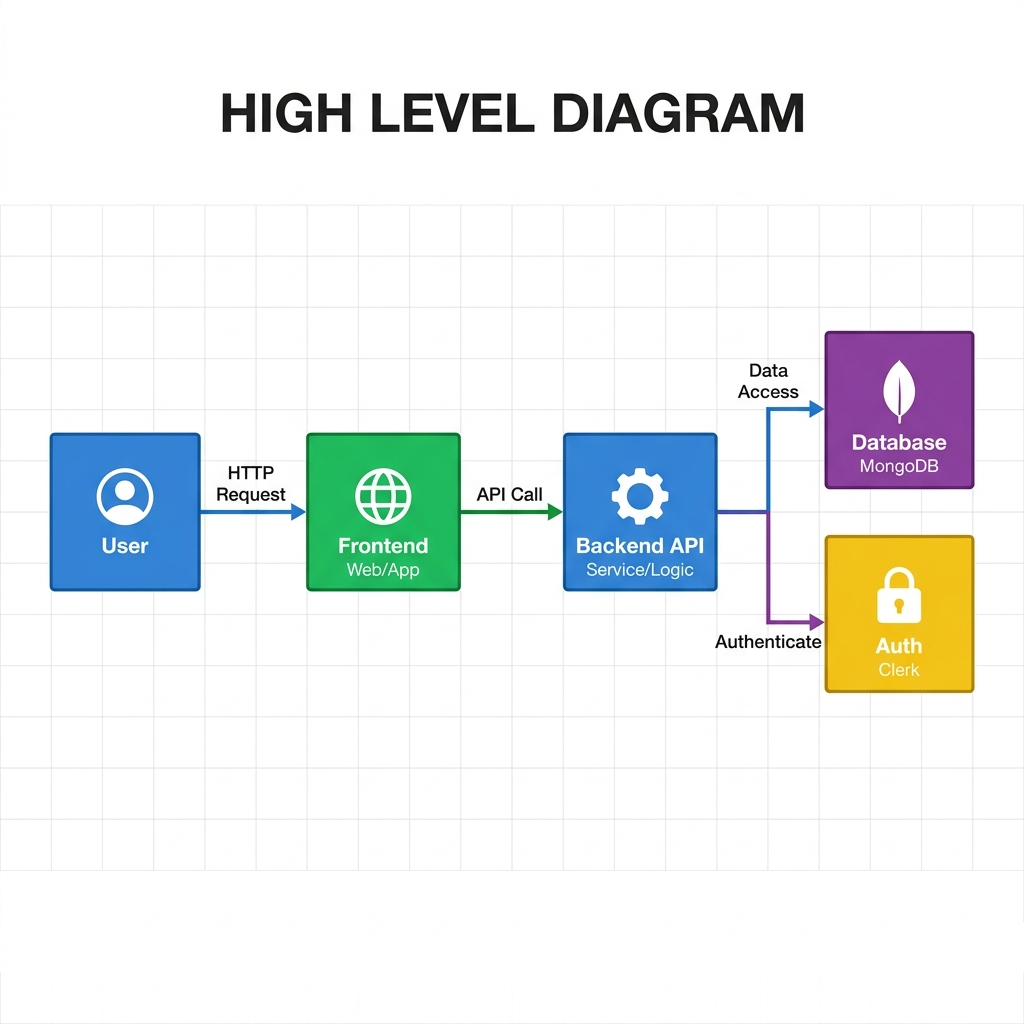
\includegraphics[width=\textwidth,keepaspectratio]{project_output/hld_ai.png}
\end{center}

\subsection{Component Map}
\begin{longtable}{>{\bfseries}p{0.18\linewidth} p{0.22\linewidth} p{0.55\linewidth}}
\toprule
Layer & File / Module & Responsibility \\ \midrule
\endfirsthead
Frontend Pages & \texttt{Dashboard.jsx} \newline \texttt{Editor.jsx} \newline \texttt{MyMaps.jsx} \newline \texttt{WorkspaceView.jsx} & Top-level page views, route endpoints \\
Canvas Core & \texttt{CanvasContainer.jsx} & Central hub; wires all hooks and renders \texttt{ReactFlow} \\
Canvas Hooks & \texttt{useCanvasState.js} \newline \texttt{useCanvasEvents.js} \newline \texttt{useCanvasActions.js} \newline \texttt{useDragReparent.js} & State sync, event handling, CRUD actions, drag reparent \\
Layout Engine & \texttt{flowUtils.js} & D3 stratify + tree layout; 3 modes; colour palette assignment \\
Node Visual & \texttt{D3StyleNode.jsx} & Renders one node bubble with inline edit, status icons, glow \\
Edge Visual & \texttt{D3BezierEdge.jsx} & Animated bezier connector between nodes \\
Backend Entry & \texttt{app.js} / \texttt{index.js} & Express middleware, CORS, auth mock, route mount \\
Routes & \texttt{mapRoutes.js} \newline \texttt{nodeRoutes.js} \newline \texttt{folderRoutes.js} & URL-to-controller mapping \\
Controllers & \texttt{mapController.js} \newline \texttt{nodeController.js} \newline \texttt{folderController.js} & HTTP req/res; delegates to services \\
Database Models & \texttt{Map.js} \newline \texttt{Node.js} \newline \texttt{Folder.js} & Mongoose schemas \\
\bottomrule
\end{longtable}

\subsection{Data Flow Diagrams (DFD)}

\subsubsection{Level 0 DFD (Context Diagram)}
\begin{center}
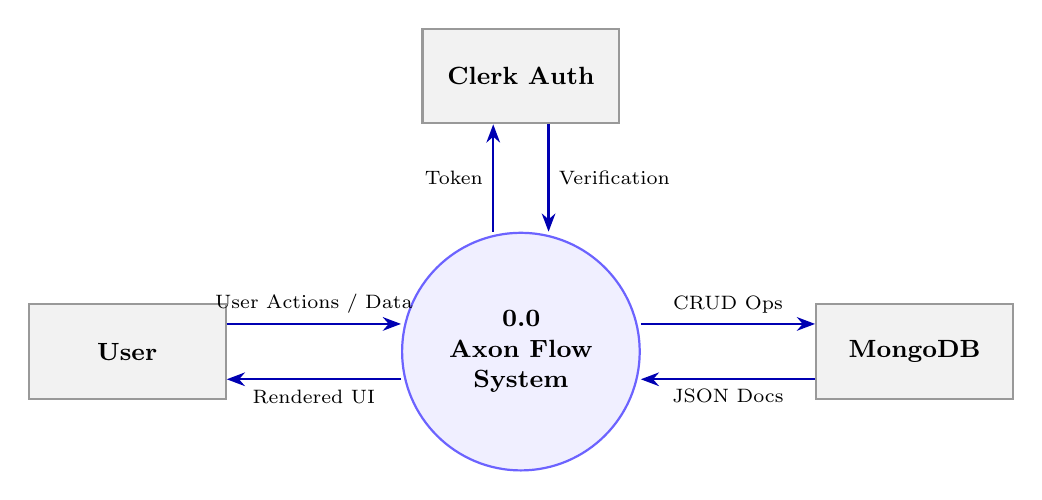
\begin{tikzpicture}[
  process/.style={circle, draw=axonpurple, thick, fill=axonpurple!10, minimum size=3cm, text width=2.5cm, align=center, font=\bfseries\small},
  ext/.style={rectangle, draw=gray!80, thick, fill=gray!10, minimum width=2.5cm, minimum height=1.2cm, align=center, font=\bfseries\small},
  flow/.style={-Stealth, thick, draw=blue!70!black},
  flowlabel/.style={font=\scriptsize, align=center}
]

% Nodes
\node[process] (system) at (0,0) {0.0\\Axon Flow\\System};
\node[ext] (user) at (-5,0) {User};
\node[ext] (clerk) at (0,3.5) {Clerk Auth};
\node[ext] (db) at (5,0) {MongoDB};

% Flows
\draw[flow] ([yshift=10pt]user.east) -- node[flowlabel, above] {User Actions / Data} ([yshift=10pt]system.west);
\draw[flow] ([yshift=-10pt]system.west) -- node[flowlabel, below] {Rendered UI} ([yshift=-10pt]user.east);

\draw[flow] ([xshift=-10pt]system.north) -- node[flowlabel, left] {Token} ([xshift=-10pt]clerk.south);
\draw[flow] ([xshift=10pt]clerk.south) -- node[flowlabel, right] {Verification} ([xshift=10pt]system.north);

\draw[flow] ([yshift=10pt]system.east) -- node[flowlabel, above] {CRUD Ops} ([yshift=10pt]db.west);
\draw[flow] ([yshift=-10pt]db.west) -- node[flowlabel, below] {JSON Docs} ([yshift=-10pt]system.east);

\end{tikzpicture}
\end{center}

\subsubsection{Level 1 DFD}
\begin{center}
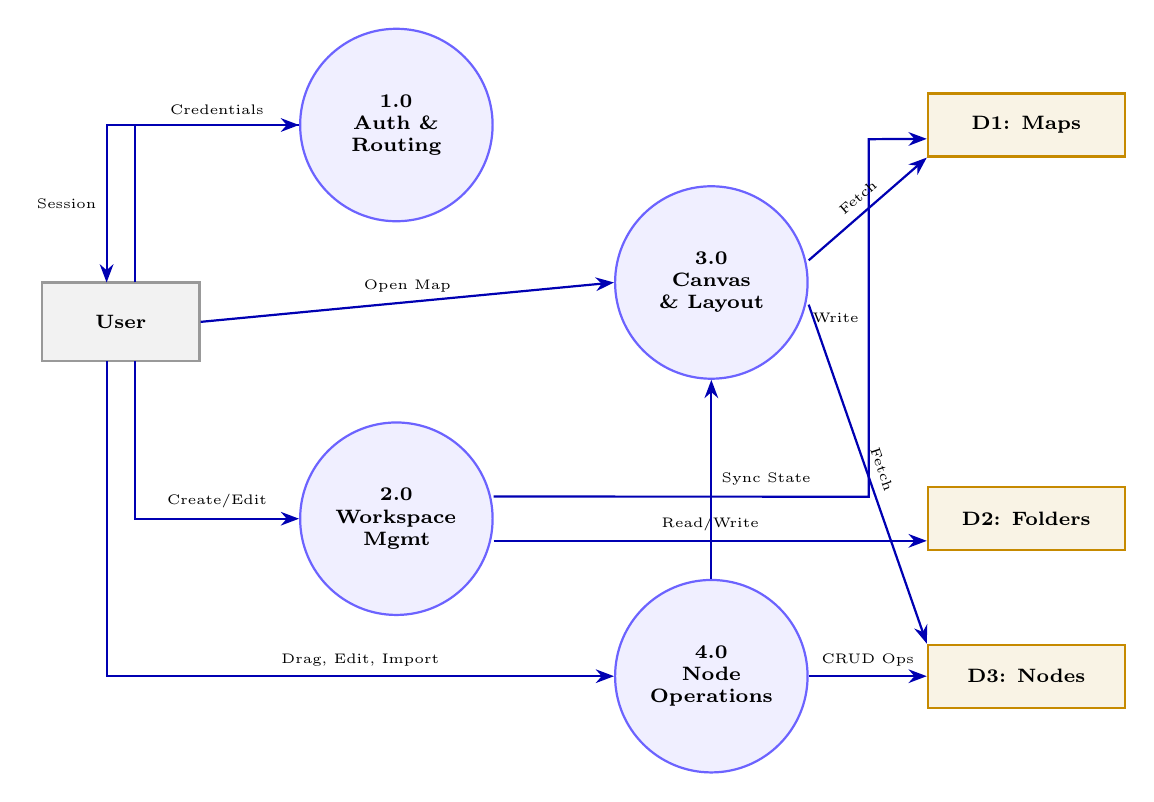
\begin{tikzpicture}[
  process/.style={circle, draw=axonpurple, thick, fill=axonpurple!10, minimum size=2.2cm, text width=2cm, align=center, font=\scriptsize\bfseries},
  store/.style={rectangle, draw=axongold, thick, fill=axongold!10, minimum width=2.5cm, minimum height=0.8cm, font=\scriptsize\bfseries, align=left, inner xsep=10pt},
  ext/.style={rectangle, draw=gray!80, thick, fill=gray!10, minimum width=2cm, minimum height=1cm, align=center, font=\scriptsize\bfseries},
  flow/.style={-Stealth, thick, draw=blue!70!black},
  flowlabel/.style={font=\tiny, align=center}
]

% External
\node[ext] (user) at (0, 0) {User};

% Processes
\node[process] (p1) at (3.5, 2.5) {1.0\\Auth \& Routing};
\node[process] (p2) at (3.5, -2.5) {2.0\\Workspace\\Mgmt};
\node[process] (p3) at (7.5, 0.5) {3.0\\Canvas \& Layout};
\node[process] (p4) at (7.5, -4.5) {4.0\\Node\\Operations};

% Stores
\node[store] (d1) at (11.5, 2.5) {D1: Maps};
\node[store] (d2) at (11.5, -2.5) {D2: Folders};
\node[store] (d3) at (11.5, -4.5) {D3: Nodes};

% Flows
\draw[flow] (0.18, 0.5) -- (0.18, 2.5) -- node[flowlabel, above] {Credentials} (p1.west);
\draw[flow] (p1.west) -- (-0.18, 2.5) -- node[flowlabel, left] {Session} (-0.18, 0.5);

\draw[flow] (0.18, -0.5) -- (0.18, -2.5) -- node[flowlabel, above] {Create/Edit} (p2.west);
\draw[flow] (-0.18, -0.5) -- (-0.18, -4.5) -- node[flowlabel, above] {Drag, Edit, Import} (p4.west);

\draw[flow] (user.east) -- node[flowlabel, above] {Open Map} (p3.west);

\draw[flow] ([yshift=8pt]p2.east) -- (9.5, -2.22) -- node[flowlabel, left] {Write} (9.5, 2.32) -- ([yshift=-5pt]d1.west);
\draw[flow] ([yshift=-8pt]p2.east) -- node[flowlabel, above] {Read/Write} ([yshift=-8pt]d2.west);

\draw[flow] ([yshift=8pt]p3.east) -- node[flowlabel, above, sloped] {Fetch} (d1.south west);
\draw[flow] ([yshift=-8pt]p3.east) -- node[flowlabel, above, sloped] {Fetch} (d3.north west);

\draw[flow] (p4.east) -- node[flowlabel, above] {CRUD Ops} (d3.west);
\draw[flow] (p4.north) -- node[flowlabel, right] {Sync State} (p3.south);

\end{tikzpicture}
\end{center}

% ════════════════════════════════════════════════════════════════════════════
\section{Detailed Data Flow — Flat DB to Canvas}

\subsection{The Core Challenge}
A mind map is a tree. Trees stored as nested documents create expensive writes (the whole document must be replaced for one change). Axon Flow stores nodes as a \textbf{flat list}; each node knows only its \texttt{parentId}. The frontend reconstructs the tree at runtime.

\subsection{Step-by-Step: Opening a Map}

\begin{center}
\begin{tikzpicture}[
  procstep/.style={rectangle, draw, thick, rounded corners=4pt, fill=axonpurple!10,
               text width=4.2cm, minimum height=0.9cm, align=center, font=\small},
  arr/.style={-Stealth, thick, axonpurple}
]
\node[procstep] (s1) {1. \textbf{API Fetch}\\\texttt{GET /api/nodes/map/:id}};
\node[procstep, right=1.2cm of s1] (s2) {2. \textbf{MongoDB Query}\\Node.find(\{mapId\})};
\node[procstep, right=1.2cm of s2] (s3) {3. \textbf{Flat JSON Array}\\returned to browser};
\node[procstep, below=0.8cm of s3] (s4) {4. \textbf{filterExpandedNodes()}\\ prune collapsed branches};
\node[procstep, left=1.2cm of s4] (s5) {5. \textbf{D3 stratify()}\\ flat list → D3 tree};
\node[procstep, left=1.2cm of s5] (s6) {6. \textbf{D3 tree() layout}\\ assign X,Y positions};
\node[procstep, below=0.8cm of s6] (s7) {7. \textbf{pushNode()}\\ build ReactFlow nodes/edges};
\node[procstep, right=1.2cm of s7] (s8) {8. \textbf{setNodes() / setEdges()}\\ React re-renders canvas};

\draw[arr] (s1)--(s2); \draw[arr] (s2)--(s3);
\draw[arr] (s3)--(s4); \draw[arr] (s4)--(s5);
\draw[arr] (s5)--(s6); \draw[arr] (s6)--(s7);
\draw[arr] (s7)--(s8);
\end{tikzpicture}
\end{center}

\subsubsection{Concrete Example}
\textbf{MongoDB stores these three documents (flat):}
\begin{lstlisting}[language=json, caption={Flat nodes stored in MongoDB}]
[
  { "_id": "NODE_101", "mapId": "MAP_001", "parentId": null,      "name": "AI Research", "x": 0,   "y": 0   },
  { "_id": "NODE_102", "mapId": "MAP_001", "parentId": "NODE_101","name": "Deep Learning","x": 300, "y": -60 },
  { "_id": "NODE_103", "mapId": "MAP_001", "parentId": "NODE_101","name": "NLP",          "x": 300, "y": 60  }
]
\end{lstlisting}

\textbf{Frontend calls \texttt{buildReactFlowData()} which runs D3 stratify:}
\begin{lstlisting}[language=javascript, caption={D3 stratify in flowUtils.js}]
const root = stratify()
  .id(d => d.id)
  .parentId(d => d.parentId)(backendNodes); // flat -> D3 hierarchy

// D3 tree() assigns .x and .y to each node in the hierarchy.
// In Horizontal mode, colX Map controls the X-axis per depth level.
// measureTextPx() ensures wide node names get wider columns.
const layout = tree().nodeSize([1, 1])
  .separation((a, b) => (hA + hB) / 2 + 40);  // dynamic gap
layout(root);
\end{lstlisting}

\textbf{Result sent to React Flow:}
\begin{lstlisting}[language=json, caption={ReactFlow node objects after layout}]
[
  { "id": "NODE_101", "type": "d3Node", "position": {"x": 0,   "y": 0},   "data": {"name": "AI Research", "depth": 0} },
  { "id": "NODE_102", "type": "d3Node", "position": {"x": 380, "y": -45}, "data": {"name": "Deep Learning","depth": 1} },
  { "id": "NODE_103", "type": "d3Node", "position": {"x": 380, "y": 45},  "data": {"name": "NLP",          "depth": 1} }
]
\end{lstlisting}

\textbf{Edge Generation \& React Flow Rendering:}
Once the nodes have their absolute positions from D3, the frontend generates React Flow \texttt{nodes} and \texttt{edges} arrays. Every child node automatically creates an edge connecting it back to its parent.

\begin{lstlisting}[language=javascript, caption={Generating Nodes and Edges for React Flow}]
const flowNodes = [];
const flowEdges = [];

// 'root' represents the D3 hierarchy tree
root.each(node => {
  // 1. Create the React Flow Node
  flowNodes.push({
    id: node.id,
    type: 'd3Node', // Maps to D3StyleNode.jsx
    position: { x: node.x, y: node.y },
    data: { name: node.data.name, depth: node.depth }
  });

  // 2. Create the Edge connecting to its parent
  if (node.parent) {
    flowEdges.push({
      id: `edge-${node.parent.id}-${node.id}`,
      source: node.parent.id, // Parent Node ID
      target: node.id,        // Child Node ID
      type: 'd3Edge',         // Maps to D3BezierEdge.jsx
      animated: true,
      style: { stroke: '#6C63FF', strokeWidth: 2 }
    });
  }
});

// React Flow consumes these arrays to render the canvas
setNodes(flowNodes);
setEdges(flowEdges);
\end{lstlisting}

\subsection{Step-by-Step: Dragging a Node}
\begin{enumerate}[noitemsep]
  \item \textbf{onNodeDrag} fires in \texttt{useDragReparent.js}. A hit-test checks if the dragged node's centre overlaps any other node bounding box (+24px padding).
  \item If a valid drop target is found (not a descendant, not current parent), it is highlighted with a blue pulsing ring (\texttt{isDropTarget}).
  \item \textbf{onNodeDragStop} fires. If a drop target exists:
    \begin{itemize}[noitemsep]
      \item \textbf{Optimistic update:} \texttt{setBackendNodes()} immediately updates \texttt{parentId} in local state → canvas re-renders instantly.
      \item \textbf{Persist:} \texttt{PATCH /api/nodes/:id \{parentId: target\}} sent to backend.
      \item \textbf{Rollback:} If the API call fails, the frontend re-fetches the full node list to revert.
    \end{itemize}
  \item If \textit{no} drop target: \texttt{PATCH /api/nodes/:id/position \{x, y\}} saves the new free-position.
\end{enumerate}

% ════════════════════════════════════════════════════════════════════════════
\section{Low-Level Design (LLD)}

\begin{center}
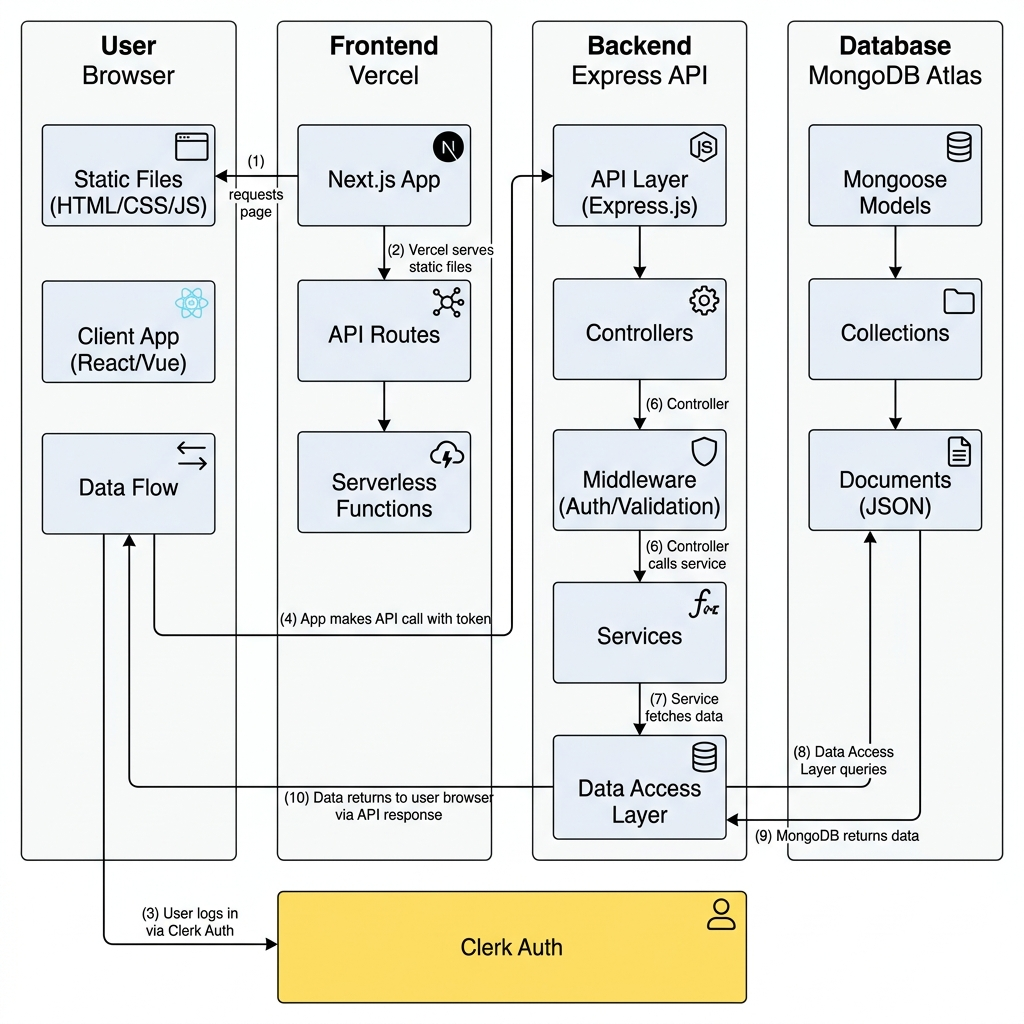
\includegraphics[width=\textwidth,keepaspectratio]{project_output/lld_ai.png}

\vspace{1cm}
\textbf{Three-Tier Architecture Diagram}
\vspace{0.5cm}

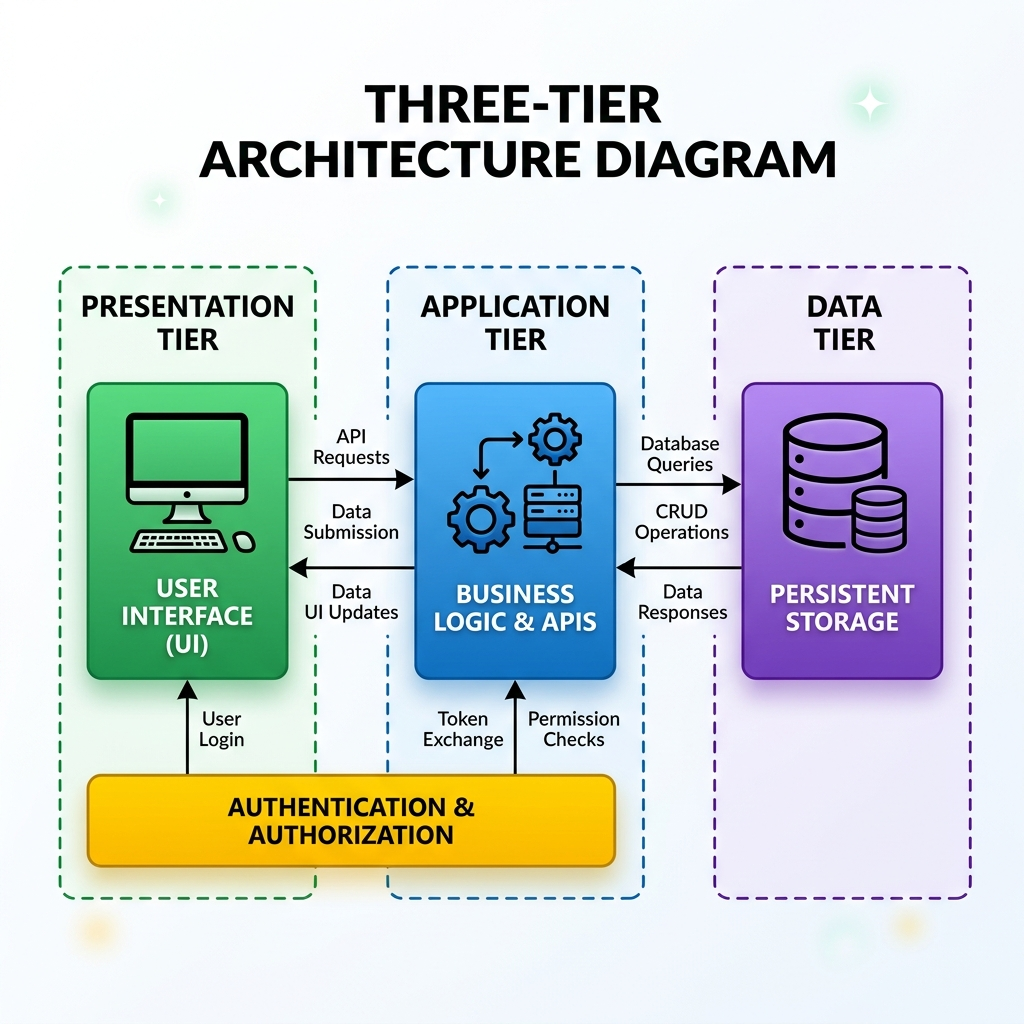
\includegraphics[width=\textwidth,keepaspectratio]{project_output/three_tier_ai.png}
\end{center}

\subsection{Database Schema}

\subsubsection{Collection: \texttt{nodes}}
\begin{center}
\begin{tabularx}{\linewidth}{>{\bfseries\ttfamily}p{0.18\linewidth} p{0.15\linewidth} X}
\toprule
Field & Type & Description \\
\midrule
mapId & ObjectId & FK → \texttt{maps} collection. Scopes node to a single map. \\
userId & String & Clerk user ID. Enforces per-user data isolation. \\
parentId & ObjectId|null & FK → \texttt{nodes} (self-ref). \texttt{null} = root node. \\
name & String & Text content of the node bubble. \\
isExpanded & Boolean & Whether children are visible on canvas. \\
notes & [String] & Deep-dive notes attached to this node. \\
links & [\{title, url\}] & Hyperlinks attached to this node. \\
files & [\{fileName, fileUrl\}] & File attachments (stored via \texttt{/api/files} upload). \\
status & String|null & Badge: reading, completed, incomplete, important, revise. \\
x, y & Number & Canvas position coordinates (for free-drag placement). \\
\bottomrule
\end{tabularx}
\end{center}

\subsubsection{Collection: \texttt{maps}}
\begin{center}
\begin{tabularx}{\linewidth}{>{\bfseries\ttfamily}p{0.2\linewidth} p{0.15\linewidth} X}
\toprule
Field & Type & Description \\
\midrule
name & String & Display name of the map. \\
userId & String & Owner's Clerk ID. \\
rootNodeId & ObjectId & Reference to the map's root node. \\
workspace & String|null & Top-level organisational label (e.g., ``Research''). \\
folderId & ObjectId|null & Optional FK → \texttt{folders} for nested organisation. \\
isFavorite & Boolean & Pinned to Favorites view. \\
isTrashed & Boolean & Soft-deleted; shown in Trash view only. \\
tags & [String] & User-defined labels for filtering. \\
lastAccessedAt & Date & Used for ``Recently Viewed'' sorting in Dashboard. \\
\bottomrule
\end{tabularx}
\end{center}

\subsubsection{Collection: \texttt{folders}}
\begin{center}
\begin{tabularx}{\linewidth}{>{\bfseries\ttfamily}p{0.18\linewidth} p{0.15\linewidth} X}
\toprule
Field & Type & Description \\
\midrule
name & String & Folder display name. \\
workspace & String & Parent workspace label (required). \\
parentId & ObjectId|null & Supports infinitely nested folder trees. \\
userId & String & Owner's Clerk ID. \\
\bottomrule
\end{tabularx}
\end{center}

\subsection{ER Diagram}
\begin{center}
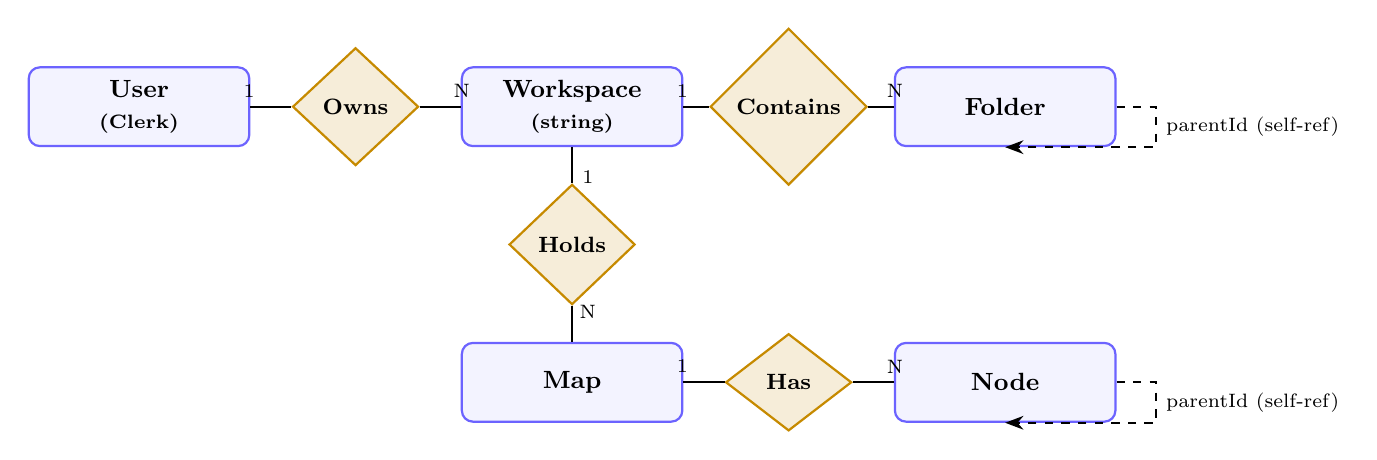
\begin{tikzpicture}[
  entity/.style={rectangle, draw=axonpurple, thick, fill=axonpurple!8,
                 rounded corners=4pt, minimum width=2.8cm, minimum height=1cm,
                 align=center, font=\bfseries\small},
  attr/.style={ellipse, draw=gray!60, fill=gray!6, minimum width=1.8cm,
               minimum height=0.7cm, font=\scriptsize\ttfamily, align=center},
  rel/.style={diamond, draw=axongold, fill=axongold!15, thick,
              minimum width=1.6cm, minimum height=0.9cm,
              align=center, font=\bfseries\footnotesize},
  line/.style={draw, thick}
]

% Entities
\node[entity] (user)   at (0,0)    {User\\{\scriptsize(Clerk)}};
\node[entity] (ws)     at (5.5,0)  {Workspace\\{\scriptsize(string)}};
\node[entity] (folder) at (11,0)   {Folder};
\node[entity] (map)    at (5.5,-3.5) {Map};
\node[entity] (node)   at (11,-3.5){Node};

% Relationships
\node[rel] (owns)  at (2.75,0)    {Owns};
\node[rel] (has)   at (8.25,0)    {Contains};
\node[rel] (holds) at (5.5,-1.75) {Holds};
\node[rel] (hasN)  at (8.25,-3.5) {Has};

% Lines
\draw[line] (user)--(owns)--(ws)--(has)--(folder);
\draw[line] (ws)--(holds)--(map);
\draw[line] (map)--(hasN)--(node);
\draw[line, dashed, -Stealth] (folder.east) -- ++(0.5,0) |- node[near start, right, font=\scriptsize]{parentId (self-ref)} (folder.south);
\draw[line, dashed, -Stealth] (node.east) -- ++(0.5,0) |- node[near start, right, font=\scriptsize]{parentId (self-ref)} (node.south);

% Cardinality labels
\node[font=\scriptsize] at (1.4,0.2) {1};
\node[font=\scriptsize] at (4.1,0.2) {N};
\node[font=\scriptsize] at (6.9,0.2) {1};
\node[font=\scriptsize] at (9.6,0.2) {N};

\node[font=\scriptsize] at (5.7,-0.9) {1};
\node[font=\scriptsize] at (5.7,-2.6) {N};

\node[font=\scriptsize] at (6.9,-3.3) {1};
\node[font=\scriptsize] at (9.6,-3.3) {N};

\end{tikzpicture}
\end{center}

\subsection{API Endpoints — Full Reference}

\subsubsection{Map Routes (\texttt{/api/maps})}
\begin{longtable}{p{0.08\linewidth} p{0.34\linewidth} p{0.52\linewidth}}
\toprule
\textbf{Method} & \textbf{Endpoint} & \textbf{Description} \\
\midrule
GET & \texttt{/maps/list} & Fetch all maps owned by authenticated user; supports query filters. \\
POST & \texttt{/maps/create} & Create a Map and atomically create its root Node. \\
PATCH & \texttt{/maps/:mapId/attributes} & Update isFavorite, isTrashed, tags, name, etc. \\
POST & \texttt{/maps/:mapId/duplicate} & Deep-clone map + all nodes with new ObjectIds. \\
PATCH & \texttt{/maps/bulk-attributes} & Update attributes on multiple maps in one call. \\
\bottomrule
\end{longtable}

\subsubsection{Node Routes (\texttt{/api/nodes})}
\begin{longtable}{p{0.08\linewidth} p{0.38\linewidth} p{0.48\linewidth}}
\toprule
\textbf{Method} & \textbf{Endpoint} & \textbf{Description} \\
\midrule
GET & \texttt{/nodes/map/:mapId} & Fetch all nodes for a map (flat array). \\
POST & \texttt{/nodes/map/:mapId} & Create a single new child node. \\
PATCH & \texttt{/nodes/:id} & Update name, isExpanded, parentId, notes, status, etc. \\
PATCH & \texttt{/nodes/:id/position} & Update x, y coordinates after free-drag. \\
DELETE & \texttt{/nodes/:id} & Recursively delete node and all descendants. \\
POST & \texttt{/nodes/bulk-update} & Batch update multiple nodes (used by copy/paste). \\
POST & \texttt{/nodes/bulk-create} & Insert an array of nodes atomically (Bulk Import). \\
\bottomrule
\end{longtable}

\subsubsection{Folder Routes (\texttt{/api/folders})}
\begin{longtable}{p{0.09\linewidth} p{0.42\linewidth} p{0.43\linewidth}}
\toprule
\textbf{Method} & \textbf{Endpoint} & \textbf{Description} \\
\midrule
GET & \texttt{/folders/workspaces/list} & Return distinct workspace names for the user. \\
PATCH & \texttt{/folders/workspaces/rename} & Rename workspace string on all maps and folders. \\
DELETE & \texttt{/folders/workspaces/:name} & Delete workspace and all its content. \\
GET & \texttt{/folders/list} & List folders by workspace and optional parentId. \\
POST & \texttt{/folders/create} & Create a new folder inside a workspace. \\
DELETE & \texttt{/folders/:id} & Recursively delete folder and all child folders/maps. \\
\bottomrule
\end{longtable}

\subsection{D3 Layout Algorithm (LLD Detail)}
The layout engine in \texttt{flowUtils.js} supports three modes:

\begin{infobox}[Horizontal Layout (Default — Column-Width Algorithm)]
\begin{enumerate}[noitemsep]
  \item \texttt{d3.stratify()} converts the flat array into a D3 hierarchy.
  \item \texttt{tree().nodeSize([1,1]).separation()} assigns abstract Y positions; gap = \texttt{(heightA + heightB) / 2 + 40px}.
  \item A \textbf{Column-Width Map} is built: for each depth level, the maximum node text width is measured using a canvas 2D context (\texttt{measureTextPx()}).
  \item Each column's X offset = previous column's X + previous column's max width + 50px gap.
  \item This prevents label overlap even with very long node names.
\end{enumerate}
\end{infobox}

\begin{infobox}[Radial Layout]
\begin{enumerate}[noitemsep]
  \item \texttt{tree().size([2*Math.PI, RADIUS])} maps the hierarchy onto a circle (angle, radius).
  \item Root placed at (0, 0); children spread at equal angular intervals.
  \item Polar $\rightarrow$ Cartesian: \texttt{x = r * cos($\theta$ - $\pi$/2)}, \texttt{y = r * sin($\theta$ - $\pi$/2)}.
\end{enumerate}
\end{infobox}

\begin{infobox}[Vertical Layout]
Standard top-down tree. \texttt{tree().nodeSize([200, 110])} — sibling gap 200px, depth gap 110px.
\end{infobox}

\subsection{Bulk Import Parser Algorithm}
Defined in \texttt{parseIndentedText()} inside \texttt{flowUtils.js}:
\begin{lstlisting}[language=javascript, caption={Bulk Import Indentation Parser}]
// Input: raw text pasted by user
// Output: flat array [{id, parentId, name}]
const stack = [{ depth: -1, id: targetParentId }]; // sentinel
lines.forEach(line => {
  const depth = countIndent(line);  // tabs=4, spaces=1
  const name  = line.trim().replace(/^[-*•]\s+/, ''); // strip bullets
  // Pop stack until we find the correct parent depth
  while (stack.length > 1 && stack[stack.length-1].depth >= depth) stack.pop();
  const parentId = stack[stack.length - 1].id;
  const id = generateId();
  newNodes.push({ id, parentId, name, isExpanded: true });
  stack.push({ depth, id });
});
\end{lstlisting}

Example input → output:
\begin{codebox}[Input text]
\begin{verbatim}
Machine Learning
    Supervised
        Regression
        Classification
    Unsupervised
\end{verbatim}
\end{codebox}
Produces: 5 node documents, each with a \texttt{parentId} pointing to the correct ancestor.

% ════════════════════════════════════════════════════════════════════════════
\section{Frontend \& Interaction Design}

\subsection{Hook Architecture}
\texttt{CanvasContainer.jsx} delegates all logic to four purpose-built hooks:
\begin{center}
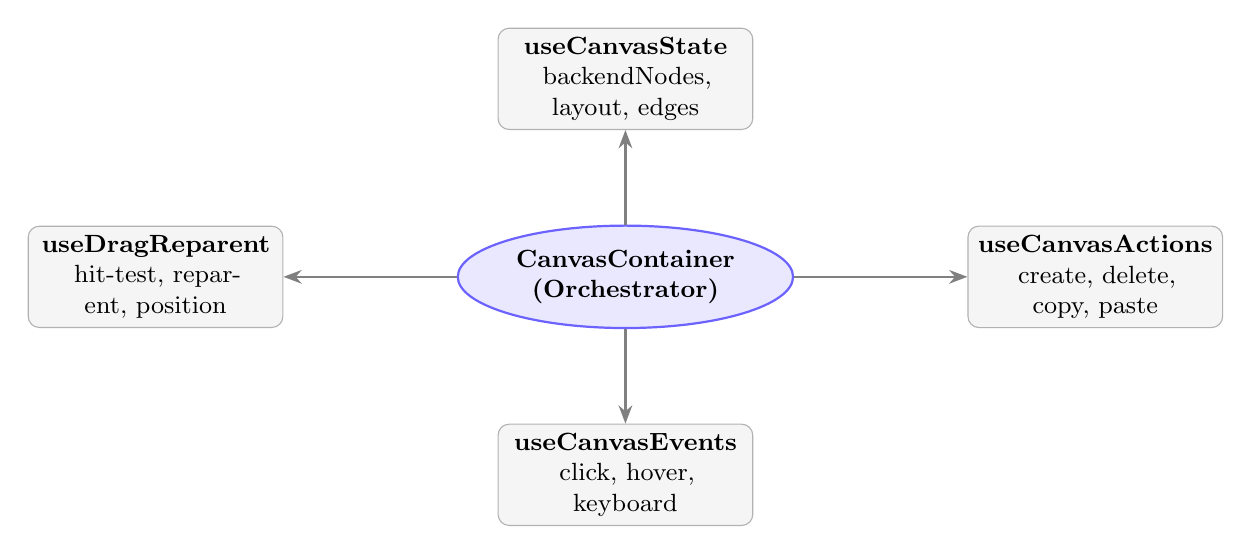
\begin{tikzpicture}[
  hub/.style={ellipse, draw=axonpurple, thick, fill=axonpurple!15,
              minimum width=3.4cm, minimum height=1.2cm, align=center, font=\bfseries\small},
  spoke/.style={rectangle, draw=gray!60, rounded corners=4pt, fill=gray!8,
                text width=3cm, minimum height=0.9cm, align=center, font=\small},
  arr/.style={-Stealth, thick, gray}
]
\node[hub] (center) {CanvasContainer\\(Orchestrator)};
\node[spoke, above=1.2cm of center]      (state)   {\textbf{useCanvasState}\\ backendNodes, layout, edges};
\node[spoke, right=2.2cm of center]      (actions) {\textbf{useCanvasActions}\\ create, delete, copy, paste};
\node[spoke, below=1.2cm of center]      (events)  {\textbf{useCanvasEvents}\\ click, hover, keyboard};
\node[spoke, left=2.2cm of center]       (drag)    {\textbf{useDragReparent}\\ hit-test, reparent, position};
\draw[arr] (center)--(state); \draw[arr] (center)--(actions);
\draw[arr] (center)--(events); \draw[arr] (center)--(drag);
\end{tikzpicture}
\end{center}

\subsection{useCanvasState: The Sync Engine}
This hook is the single source of truth. Whenever \texttt{backendNodes}, \texttt{layoutMode}, or \texttt{colorPalette} changes, a \texttt{useEffect} fires and:
\begin{enumerate}[noitemsep]
  \item Calls \texttt{filterExpandedNodes()} to prune collapsed subtrees.
  \item Calls \texttt{buildReactFlowData()} to recompute positions.
  \item Enriches each node with runtime callbacks: \texttt{onToggle}, \texttt{onDraftConfirm}, \texttt{onDraftCancel}.
  \item Calls \texttt{setNodes()} and \texttt{setEdges()} to push into React Flow.
\end{enumerate}

\subsection{D3StyleNode: The Node Visual Component}
Each node on canvas is rendered by \texttt{D3StyleNode.jsx}. Key design decisions:
\begin{itemize}[noitemsep]
  \item \textbf{Dynamic width:} Node width is calculated using a Canvas 2D \texttt{measureText()} call — no fixed widths.
  \item \textbf{Inline editing:} Double-click flips the node into an \texttt{<input>} field. \texttt{Enter} confirms, \texttt{Escape} cancels.
  \item \textbf{Glow ring:} On hover or selection, a coloured glow ring (matching branch colour) appears via CSS \texttt{box-shadow}.
  \item \textbf{Drop-target pulse:} When a node is dragged over, a pulsing blue ring animates via \texttt{pulseRing} keyframe.
  \item \textbf{Status icons:} Lucide React icons rendered based on the \texttt{status} field value.
\end{itemize}

\subsection{Keyboard Interaction Map}
\begin{center}
\begin{tabular}{lll}
\toprule
\textbf{Key} & \textbf{Condition} & \textbf{Action} \\
\midrule
\texttt{Tab} & Node focused & Create child node (open input as draft) \\
\texttt{Enter} & Node focused & Create sibling node \\
\texttt{F2} & Node focused & Rename node (inline edit) \\
\texttt{Delete} & Node focused & Delete node + all descendants (with confirm) \\
\texttt{Ctrl+C} & Node focused & Copy node branch to clipboard \\
\texttt{Ctrl+V} & Node focused & Paste branch as children \\
\texttt{Paste} & Canvas focused, text in clipboard & Trigger Bulk Import parser \\
\texttt{Right-click} & Any node & Open context menu (FloatingToolbar) \\
\bottomrule
\end{tabular}
\end{center}

\subsection{Context Menu — FloatingToolbar}
Right-clicking any node opens a \texttt{FloatingToolbar} positioned at cursor coordinates, offering:
Rename, Add Child, Delete, Copy, Paste, Bulk Import, Open Notes, Open Links, Open Files, Open AI.

% ════════════════════════════════════════════════════════════════════════════
\section{Non-Functional Requirements}

\begin{longtable}{>{\bfseries}p{0.06\linewidth} p{0.14\linewidth} p{0.57\linewidth} p{0.15\linewidth}}
\toprule
ID & Category & Requirement & Target \\
\midrule
\endfirsthead
NFR-01 & Performance & Canvas renders map with 500 nodes without dropping below 30 FPS & $\geq$30 FPS \\
NFR-02 & Performance & API response for \texttt{GET /nodes/map/:id} for a 500-node map & $<$300ms \\
NFR-03 & Performance & Bulk Import of a 200-line indented text file & $<$1s \\
NFR-04 & Security & All protected routes return HTTP 401 without a valid \texttt{userId} & Always \\
NFR-05 & Security & Users cannot access maps owned by other \texttt{userId}s & Always \\
NFR-06 & Security & CORS configured to allow only the production frontend domain & Always \\
NFR-07 & Reliability & Reparent drag failure triggers automatic rollback from backend re-fetch & Always \\
NFR-08 & Usability & Keyboard shortcuts (Tab, Enter, F2, Delete) are functional on all nodes & Always \\
NFR-09 & Usability & Inline node editing activates within 50ms of double-click & $<$50ms \\
NFR-10 & Scalability & Adding a new layout mode requires only changes to \texttt{flowUtils.js} & Isolated \\
\bottomrule
\end{longtable}

% ════════════════════════════════════════════════════════════════════════════
\section{Testing Requirements}

\subsection{Strategy}
\begin{itemize}[noitemsep]
  \item \textbf{Unit Tests (Jest):} Pure functions — \texttt{parseIndentedText()}, \texttt{buildReactFlowData()}, \texttt{filterExpandedNodes()}, \texttt{isDescendantOf()}.
  \item \textbf{Integration Tests (Supertest):} All REST endpoints with mock \texttt{userId} injection.
  \item \textbf{E2E Tests (Cypress/Playwright):} Full user journeys on a running dev server.
\end{itemize}

\subsection{Key Test Cases}
\begin{longtable}{p{0.09\linewidth} p{0.37\linewidth} p{0.47\linewidth}}
\toprule
\textbf{ID} & \textbf{Scenario} & \textbf{Expected Result} \\
\midrule
\endfirsthead
TC-01 & \textit{Bulk import of 5-level indented text} & 5-level tree created with correct parentId chain \\
TC-02 & \textit{Drag a node onto its own descendant} & Drop target highlighted is skipped; no reparent \\
TC-03 & \textit{Drag reparent succeeds} & \texttt{parentId} updated in DB; canvas re-renders instantly \\
TC-04 & \textit{API call fails during reparent} & Frontend reverts to pre-drag state by re-fetching \\
TC-05 & \textit{GET /nodes/map/:id by non-owner} & HTTP 401 returned \\
TC-06 & \textit{Create map} & Map + root node both created; \texttt{rootNodeId} is set \\
TC-07 & \textit{Delete node with 3 descendants} & All 4 nodes removed from DB; canvas updates \\
TC-08 & \textit{Collapse a node (\texttt{isExpanded=false})} & Children hidden from canvas; expand restores them \\
TC-09 & \textit{Switch layout from Horizontal to Radial} & Canvas re-renders in radial polar layout \\
TC-10 & \textit{Node with notes shows [Icon]\ badge} & Badge visible in D3StyleNode display text \\
\bottomrule
\end{longtable}

% ════════════════════════════════════════════════════════════════════════════
\section{Deployment \& Planning}

\subsection{Deployment Architecture}
\begin{center}
\begin{tabular}{lll}
\toprule
\textbf{Component} & \textbf{Platform} & \textbf{Notes} \\
\midrule
Frontend (React/Vite) & Vercel & Auto-deploy from Git; CDN-served globally \\
Backend (Express) & Render / Railway & Node.js v18 Docker container, port 5000 \\
Database & MongoDB Atlas & Shared M0 (free) or Serverless tier \\
Auth & Clerk & Free tier, JWT-based \\
File Storage & TBD (Cloudinary / S3) & For \texttt{files[]} attachments per node \\
\bottomrule
\end{tabular}
\end{center}

\subsection{Development Milestones}
\begin{center}
\begin{tabular}{llll}
\toprule
\textbf{Phase} & \textbf{Duration} & \textbf{Deliverable} & \textbf{Status} \\
\midrule
Architecture & 1 week & Repo, schema, route skeleton & \textcolor{codegreen}{Done} \\
Backend Core & 1 week & All REST endpoints + services & \textcolor{codegreen}{Done} \\
Canvas Engine & 2 weeks & React Flow + D3 layout + 3 modes & \textcolor{codegreen}{Done} \\
Bulk Import & 1 week & Parser + bulk-create endpoint & \textcolor{codegreen}{Done} \\
Dashboard UI & 1 week & Dashboard, MyMaps, Workspace & \textcolor{codegreen}{Done} \\
Rich Nodes & 1 week & Notes, Links, Files, Status & In Progress \\
AI Features & 2 weeks & Node generation via LLM API & Planned \\
E2E Testing & 1 week & Cypress test suite & Planned \\
Production & 1 week & Vercel + Render deploy & Planned \\
\bottomrule
\end{tabular}
\end{center}

\subsection{Future Enhancements}
\begin{enumerate}[noitemsep]
  \item \textbf{AI Node Generation:} Select a node and invoke an LLM API to auto-generate a list of relevant child topics.
  \item \textbf{Real-time Collaboration:} WebSocket layer (Socket.io) so multiple users can edit the same map simultaneously with live cursors.
  \item \textbf{Export:} Download map as a high-resolution PNG, PDF, or Markdown outline.
  \item \textbf{Templates:} Pre-built map structures (SWOT Analysis, Project Plan, Study Schedule) loaded via \texttt{bulk-create}.
  \item \textbf{Deadline/Reminders:} Add a \texttt{deadline} Date field to nodes and surface overdue items in the Dashboard.
\end{enumerate}

% ════════════════════════════════════════════════════════════════════════════
\section{Conclusion}
Axon Flow is architected around one central insight: storing mind-map nodes as a \textit{flat, independently updatable list} in MongoDB — rather than as deeply nested documents — provides superior performance for both reads and writes, without sacrificing the rich, hierarchical user experience.

The frontend resolves this flat representation into a beautiful visual tree at runtime using D3-Hierarchy's battle-tested layout algorithms, React Flow's performant Virtual DOM graph, and four purpose-built hooks that cleanly separate state, events, actions, and drag logic.

The result is a system that feels instant to the user, is easy to extend for developers, and is ready to grow into an AI-assisted, collaborative knowledge-mapping platform.

% ════════════════════════════════════════════════════════════════════════════
\section*{Appendix — Technology Stack}
\begin{longtable}{>{\bfseries}p{0.28\linewidth} p{0.15\linewidth} p{0.5\linewidth}}
\toprule
Technology & Version & Role \\
\midrule
\endfirsthead
React & 18 & UI framework and Virtual DOM rendering \\
@xyflow/react (React Flow) & 12+ & Interactive node-graph canvas \\
d3-hierarchy & 3 & Tree layout (stratify, tree) \\
Vite & 5 & Frontend build tool (HMR, fast build) \\
Node.js & 18 & Backend JavaScript runtime \\
Express.js & 4 & REST API framework \\
MongoDB Atlas & 6 & Cloud NoSQL database \\
Mongoose & 7 & ODM for MongoDB schema and queries \\
Clerk & latest & Authentication, JWT, OAuth \\
Lucide React & latest & Status icons in node component \\
TailwindCSS & 3 & Dashboard and page-level styling \\
\bottomrule
\end{longtable}

% ════════════════════════════════════════════════════════════════════════════
\section{Project Outputs \& Screenshots}

\begin{figure}[H]
    \centering
    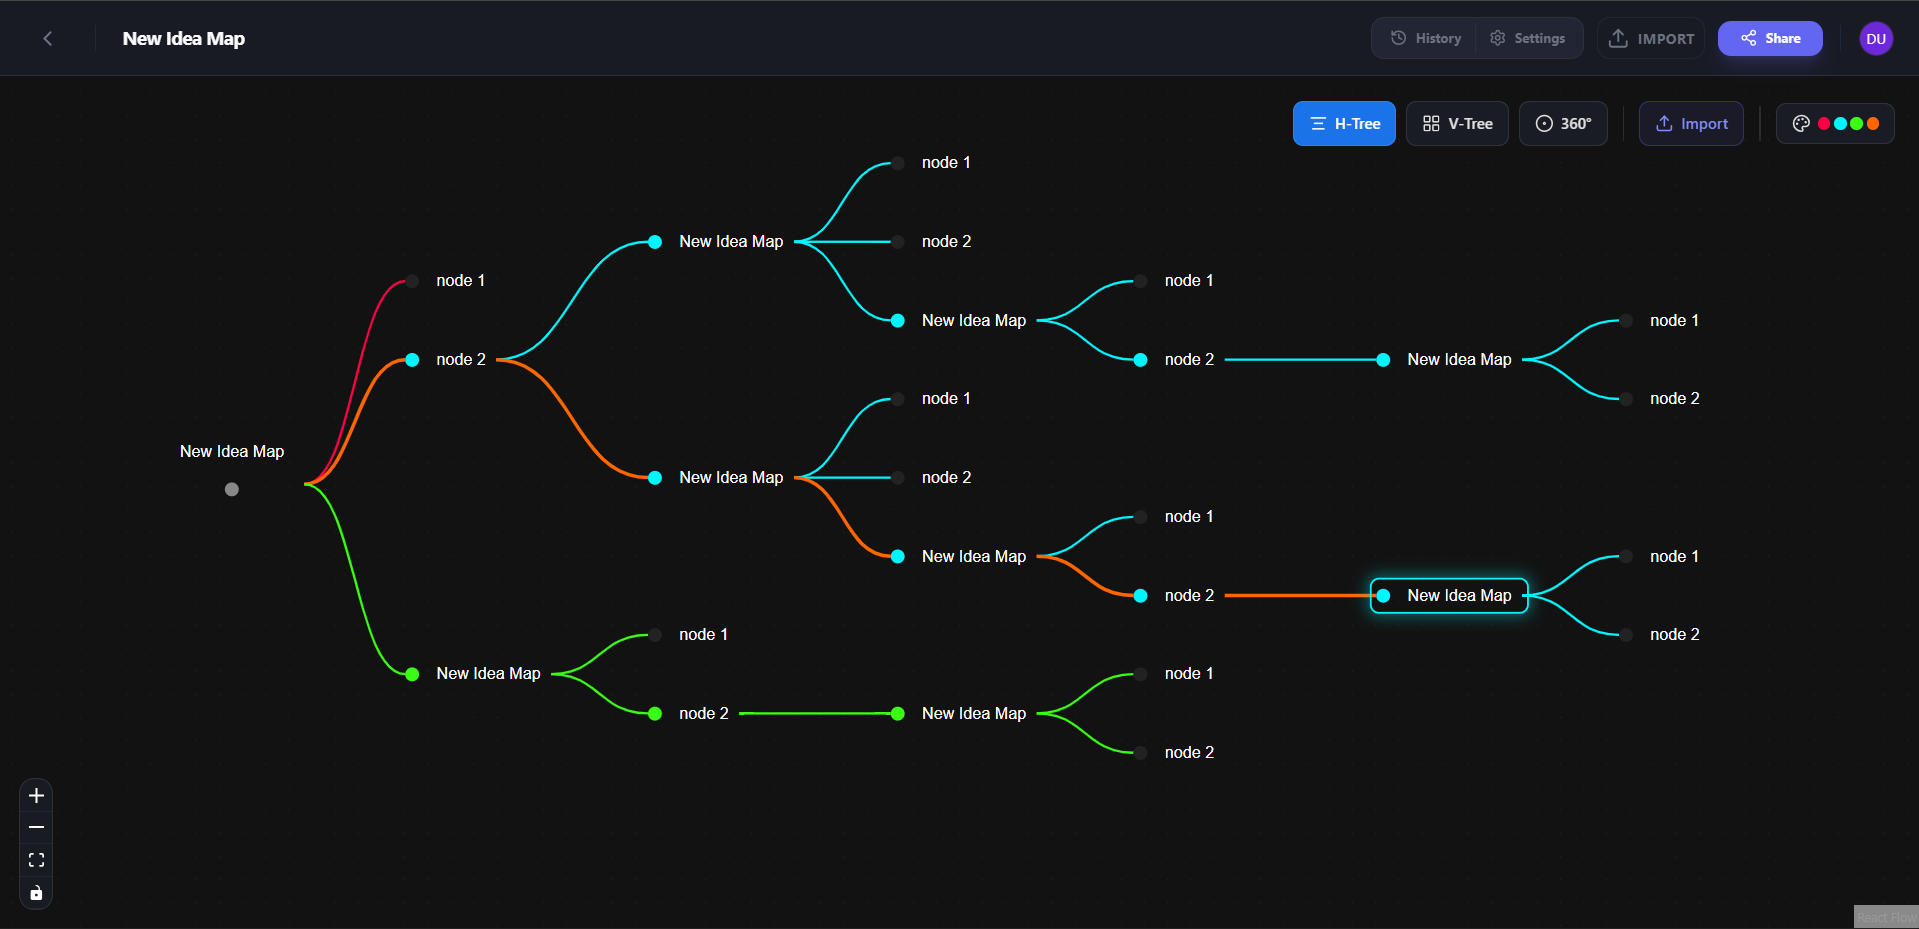
\includegraphics[width=\textwidth, keepaspectratio]{project_output/screen1.png}
    \caption{AxonFlow Interface - Workspace \& Dashboard}
\end{figure}

\vspace{1cm}

\begin{figure}[H]
    \centering
    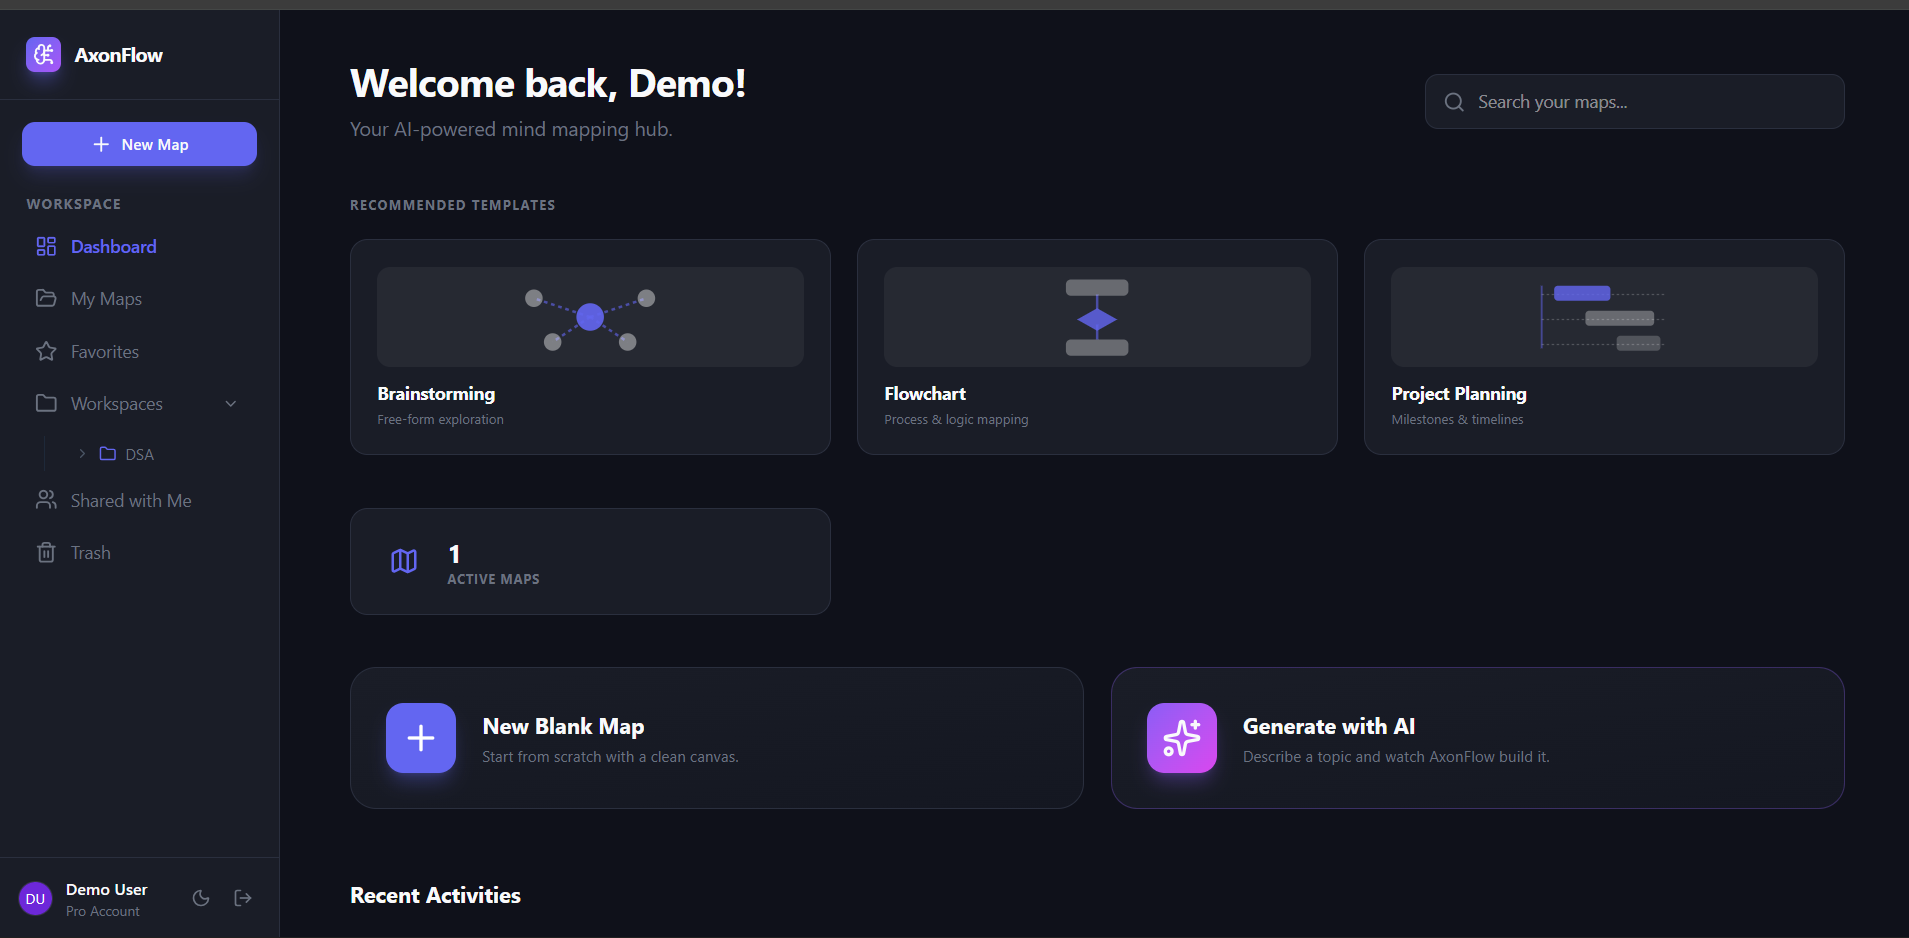
\includegraphics[width=\textwidth, keepaspectratio]{project_output/screen2.png}
    \caption{AxonFlow Interface - Mind Map Canvas Editor}
\end{figure}

\vspace{1cm}

\begin{figure}[H]
    \centering
    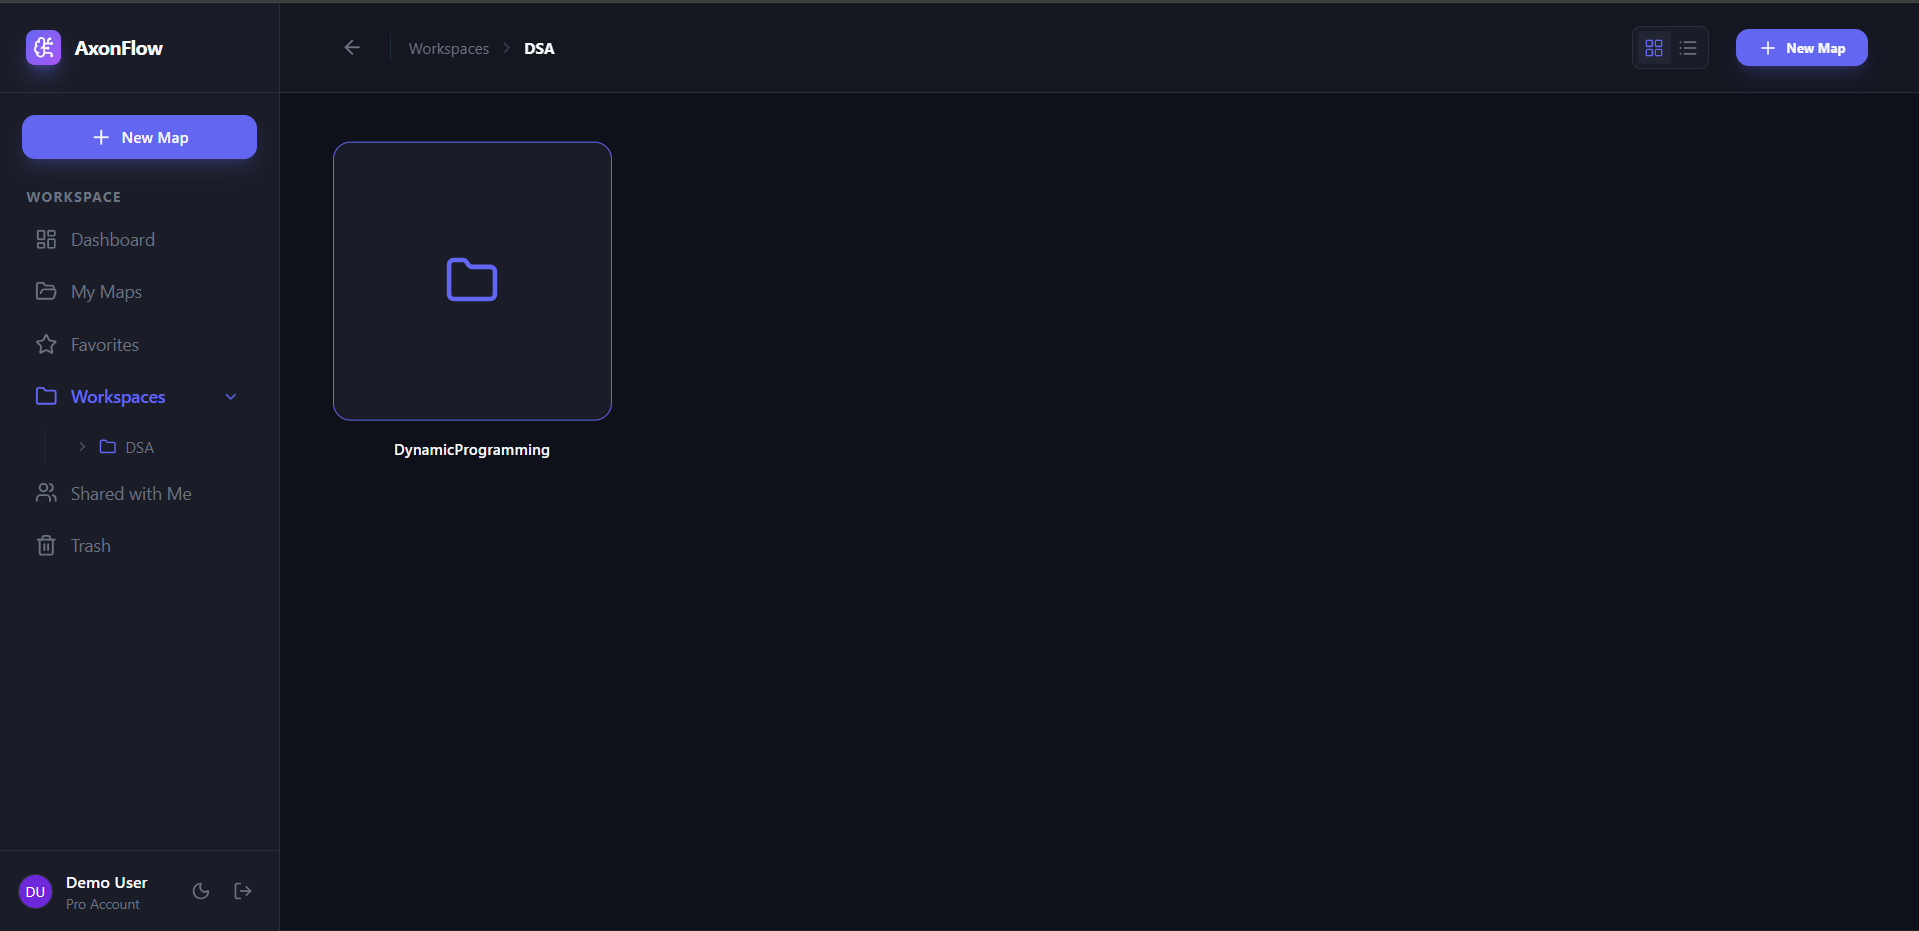
\includegraphics[width=\textwidth, keepaspectratio]{project_output/screen3.png}
    \caption{AxonFlow Interface - Node Details and Panels}
\end{figure}

\end{document}

